\chapter{Introducción Matematica}

%    En este capitulo se van a explicar los conceptos matemáticos utilizados con un ejemplo, para luego aplicarlos al estudio del caso que nos interesa. Se va a calcular la función $\zeta _A (s)$ mediante distintas técnicas, calculando asintóticamente los autovalores, y luego ponerlos en la definición o en el Heat Kernel, y luego se procedió a utilizar el calculo completo
    
    En este capitulo se van a explicar los concepctos matemátocps utilizados con varios ejemplos, para luego poder aplicarlos al operador diferencial que nos interesa, se va a calcular la funcion $ \zeta _A (s) $ de dos maneras distintas y luego se van a calcular sus respectivas energías de vacio.

\section{Ejemplos Sencillos}

En estudiaran los autovalores del operador diferencial $A = - \partial ^2 _x$ con distintas condiciones de contorno:

\subsection{Dirichlet}

El operador $A$ estara dado por : 

\begin{equation}
\begin{array}{c}
    A \phi (x) = - \partial ^2 _x \ \phi (x)  \\
    \phi (0) = \phi(L) = 0 \\ 
\end{array}
\end{equation}

Cuyos autovalores estan dados por  : 

\begin{equation}
\begin{array}{c}
	\lambda _n = \left( \frac{n \pi }{L} \right) ^2 \\
	n > 0
\end{array}
\end{equation}

La funcion $\zeta _A (s)$ queda determinada por:

\begin{equation}
\zeta _A (s) = 
\sum _{n=1} ^{\infty} \lambda ^{-2s} =  
\left( \frac{\pi}{L} \right) ^{-2s} \sum _{n=1} ^{\infty} n ^{-2s} = 
\left( \frac{\pi}{L} \right() ^{-2s} \zeta (2s)
\end{equation}

\subsection{Neuman}

El operador $A$ estara dado por : 

\begin{equation}
\begin{array}{c}
    A \phi (x) = - \partial ^2 _x \ \phi (x)  \\
    \phi ' (0) = \phi ' (L) = 0 \\ 
\end{array}
\end{equation}

Cuyos autovalores estan dados por  : 

\begin{equation}
\begin{array}{c}
	\lambda _n = \left( \frac{n \pi }{L} \right) ^2 \\
	n \geq 0
\end{array}
\end{equation}

La funcion $\zeta _A (s)$ queda determinada por:

\begin{equation}
\zeta _A (s) = 
\sum _{n=0} ^{\infty} \lambda ^{-2s} =  
\left( \frac{\pi}{L} \right) ^{-2s} \sum _{n=1} ^{\infty} n ^{-2s} = 
\left( \frac{\pi}{L} \right) ^{-2s} \zeta (2s)
\end{equation}

\subsection{Periodicas}

El operador $A$ estara dado por : 

\begin{equation}
\begin{array}{c}
    A \phi (x) = - \partial ^2 _x \ \phi (x)  \\
    \phi (0) = \phi (L)  \\ 
\end{array}
\end{equation}

Cuyos autovalores estan dados por  : 

\begin{equation}
\begin{array}{c}
	\lambda _n = \left( \frac{2 n \pi }{L} \right) ^2 \\
	n \geq 0
\end{array}
\end{equation}

La funcion $\zeta _A (s)$ queda determinada por:

\begin{equation}
\zeta _A (s) = 
\sum _{n=0} ^{\infty} \lambda ^{-2s} =  
\left( \frac{2 \pi}{L} \right) ^{-2s} \sum _{n=1} ^{\infty} n ^{-2s} = 
\left( \frac{2 \pi}{L} \right) ^{-2s} \zeta (2s)
\end{equation}

\section{Condiciones de Contorno Mixtas}

\begin{equation}
\begin{array}{c}
    A \phi (x) = - \partial ^2 _x \ \phi (x)  \\
    \phi (0) = 0 \\ 
    \partial _x \phi (L) + \gamma \phi (L) = 0
\end{array}
\end{equation}

Donde las condiciones de contorno me fijan un espectro autovalores $\lambda > 0 $, que está dado cualquiera de las dos ecuaciones equivalentes: 

\begin{equation}
\begin{array}{cc}
    \frac{\lambda}{\gamma}  \ Cos( L \lambda ) +   Sin( L \lambda ) = 0 \\
    \frac{\lambda}{\gamma}  + Tg(\lambda L )  = 0 
\label{autovalores}
\end{array}
\end{equation}

Una vez obtenidos los autovalores el siguiente paso es calcular la funcion $\zeta$ definida por:

\begin{equation}
    \zeta _ {A } (s) = \sum_{n = 1} ^{ \infty } \lambda _n ^ {-s}
\end{equation}

Al no poder encontrar explícitamente los autovalores se proceden a distintas técnicas para hallar distintas aproximaciones de la función $\zeta _A (s)$

\section{Calculo Asintótico de los autovalores}


Haciendo el cambio de variables $\mu = \lambda L$ y $\theta = \gamma L $ las ecuaciones (\ref{autovalores}) se pueden expresar de la forma:

\begin{equation}
\begin{array}{c}
    Tg[\mu] + \frac{\mu}{\theta} = 0 \\
    \frac{\mu}{\theta} Cos[\mu] + Sin[\mu] = 0
\end{array}
\label{eq.asintota}
\end{equation}

Tal como se puede ver en la figura (\ref{fig:Dibujo}), los autovalores $\mu _n$ tienden a pegarse a la asíntota vertical de $ Tg [ \mu ] $ a medida que $\mu _n$ se hace cada vez mas grande.

\begin{figure}
    \centering
    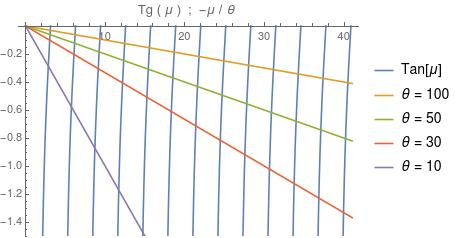
\includegraphics[scale=0.3]{Dibujo.jpg}
    \caption{Aquí se busca encontrar los terminos que no se anulan a n = $\infty$ del desarrollo asintotico de autovalores de la ecuacion (\ref{eq.asintota}) }
    \label{fig:Dibujo}
\end{figure}

Se puede ver entonces de los autovalores $\mu _n$ se pueden descomponer en una parte correspondiente a las asíntotas verticales de $Tg(x)$ mas una corrección que tiende a cero a medida que n tiende a $\infty$

\begin{equation}
\begin{array}{c}
    \mu _n = n \pi + \frac{\pi}{2} + \epsilon _n \\
    Donde \ \epsilon _n \rightarrow{0} \ si \ cuando \ n \rightarrow{0}
\end{array}
\label{eq.mu}
\end{equation}


conocer $\epsilon _n $ es equivalente a resolver la ecuación (\ref{eq.asintota}), la cual no puede resolverse analíticamente, en vez de eso voy a obtener un desarrollo de $\epsilon _n $ para $n \rightarrow \infty$.

voy a intesertar (\ref{eq.mu}) en la segunda ecuacion de (\ref{eq.asintota}) y desarrollar alrededor de $\epsilon \rightarrow{0}$ obteniendo:

\begin{equation}
\begin{array}{c}
    Sin[ n \pi + \frac{\pi}{2} + \epsilon _n ] = 
    - \frac{\mu _n}{\theta}  \ Cos[ n \pi + \frac{\pi}{2} + \epsilon _n ]  \\
 \\

         \sum _{p=0} ^{\infty} \frac{(-1) ^n  \epsilon ^{2 p }}{(2p)!} 
    =  \frac{-1}{\theta}  \ (n \pi + \frac{\pi}{2} + \epsilon ) \
     \sum _{p=0} ^{\infty} \frac{(-1) ^n \epsilon ^{2 p + 1}}{(2p+1)!} 
\end{array}
\end{equation}


Donde acomodando la igualdad, obtengo la ecuacion :

\begin{equation}
    1 = \sum _{p=1} ^{\infty} \epsilon ^{2p+2} \ (-1) ^p
    \left( 
    \frac{1}{(2p+2)!} + \frac{1}{\theta} \frac{(1 )}{(2p+1)!} 
    \right ) +
    \frac{1}{\theta} \left(n \pi + \frac{\pi}{2} \right)
    \sum _{p=0} ^{\infty} \frac{(-1) ^p \epsilon ^{2p+1}}{(2p+1) !}
\label{igualdad epsilon}
\end{equation}

Suponiendo que $\epsilon _n $ tiene un desarrollo en serie de la forma (\ref{eq.epsilon}).

\begin{equation}
    \epsilon = 
    \frac{\epsilon ^{(1)}}{n}  + 
    \frac{\epsilon ^{(2)}}{n ^2}  + 
    \frac{\epsilon ^{(3)}}{n ^3}  + ...
\label{eq.epsilon}
\end{equation}


Insertando este desarrollo de $\epsilon$ en la ecuación (\ref{igualdad epsilon}), e igualando orden a orden se obtiene, para los primeros ordenes de $\epsilon$:

\begin{equation}
    \epsilon  = \frac{\theta}{n \pi} 
     - \frac{ \theta}{2 \pi n ^2 } 
    + \frac{\theta}{n^3 \pi} 
        \left( \frac{1}{4} - 
        \frac{\theta ^2}{2 \pi ^2} -
        \frac{\theta}{\pi ^2}
        \right) 
\label{epsilons}
\end{equation}

Una vez obtenido el desarrollo de $\mu _n $ puedo calcular $\lambda _n = \frac{\mu _n }{L}  $ 



\begin{equation}
    \lambda _n = 
    \frac{1}{L}
    \left(
    \alpha n + 
    \beta + 
    \frac{\gamma}{n} +
    \frac{\delta}{n ^2} +
    \frac{\eta}{n^3} +
    O(\frac{1}{n^4} ) 
    \right)
\end{equation}
    
Donde $\alpha, \beta , ... $ quedan escritos en funcion de los $\epsilon ^{(1)},\epsilon^{(2)}, ... $ ; 
Luego se calcula la funcion $\zeta _A (s) $ utilizando el desarrollo asintotico de los autovalores.
    
\begin{equation}
\begin{array}{cc}
    \zeta _{A} (s) =  \sum _{n=1} ^{\infty} \lambda _n ^ {-2 s} =
    L ^{2s}
    \sum _{n=1} ^{\infty} 
    \left(
    \alpha n + 
    \beta + 
    \frac{\gamma}{n} +
    \frac{\delta}{n ^2} +
    \frac{\eta}{n^3} +
    O( \frac{1}{n ^{4} }  )
    \right) ^{-2 s} = \\
    ( \frac{L}{\alpha} ) ^{2s}    
    \sum _{n=1} ^{\infty} 
    n ^{- 2 s} 
    \left(
    1 +     
    \underbrace{
        \frac{\beta}{\alpha n} + 
        \frac{\gamma}{\alpha n^2} +
        \frac{\delta}{\alpha n ^3} +
        \frac{\eta}{\alpha n^4} +
        O(\frac{1}{n ^{5}} ) } _{ \chi _n}
    \right ) ^{-2 s}
\end{array}
\end{equation}

Para calcular esta serie voy a hacer un desarrollo binomial alrededor de $\chi _n \rightarrow{0} $ 

\begin{equation}
\begin{array}{c}
\zeta _{A} (s) = 
( \frac{L}{\alpha} ) ^{2s}
\sum _{n=1} ^{\infty}
  n  ^{-2 S} \\
(
1 - 2 s \chi _n + 2 s(s+1) \frac{\chi _n ^2}{2} - 2s(2s+1)(2s+2) \frac{ \chi _n ^3}{3!}  + \\ 
2s(2s+1)(2s+2)(2s+3) \frac{\chi ^4 _n}{4!}
+ O( \frac{1}{n ^5}) )

\end{array}
\end{equation}

Donde hay que tener en cuenta que cada termino $\chi _{n} ^{m} $ contribuye al orden mas bajo en la sumatoria en una potencia $\frac{1}{n ^m}$.


Calculando explicitamente cada termino, obtengo:

\begin{equation}
\sum _{n=1} ^{\infty} n ^{-2 s} = \zeta (2s)
\end{equation}


\begin{equation}
\begin{array}{c}
\begin{array}{c}
\sum _{n=1} ^{\infty}
 n  ^{-2 S}  \chi _n =  \\
\frac{\beta}{\alpha} \zeta (2s+1) + 
\frac{\gamma}{\alpha} \zeta(2s+2) + 
\frac{\delta}{\alpha} \zeta(2s+3) +
\frac{\eta}{\alpha} \zeta (2s+4) + 
\sum _{n=1} ^{\infty} n ^{-2s} O(\frac{1}{n ^5})
\end{array}
\end{array}
\end{equation}

\begin{equation}
\begin{array}{c}
    \sum _{n=1} ^{\infty}
    n   ^{-2 S} \chi _n ^2 = \\ 
    \frac{\beta ^2}{\alpha ^2} \zeta(2s+2) +
    \frac{2 \gamma \beta }{\alpha} \zeta (2s+3) + 
    \left( \frac{2 \beta \delta}{\alpha ^2} + \frac{\gamma ^2}{\alpha ^2} \right) \zeta (2s+4) + 
    \sum _{n=1} ^{\infty} n ^{-2s} O( \frac{1}{n^s} )
\end{array}
\end{equation}

\begin{equation}
\begin{array}{cc}
    \sum _{n=1} ^{\infty} 
    n ^{-2 S} \chi _n ^3 =
    \frac{\beta ^3}{\alpha ^3} \zeta (2s+3) + 
    \frac{3 \gamma \beta ^2}{\alpha ^3} \zeta (2s+4)
    + \sum _{n=1} ^{\infty} n ^{-2s} O( \frac{1}{n ^5} )
    
\end{array}
\end{equation}

\begin{equation}
\sum _{n=1}  ^{\infty} n ^{-2s} \chi _n ^4 = \\
\frac{\beta ^4}{\alpha ^4} \zeta (2s+4) + 
\sum _{n=1} ^{\infty} n ^{-2s} O( \frac{1}{n ^5} )
\end{equation}



Una vez calculados todos los terminos los sumo y saco factor común cada $\zeta( 2s+n )$


Obteniendo como resultado 

\begin{equation}
    \zeta _A (s) = 
    C _s \ \zeta (s) +
    C _{s+1} \ \zeta (s+1) + 
    C _{s+2} \ \zeta (s+2) +
    C _{s+3} \ \zeta (s+3) + 
    C _{s+4} \ \zeta (s+4) + ....
\end{equation}

Se puede ver que el resultado esta expresado como suma de funciones $\zeta (s+n)$ acompañados de unos argumentos $C_{s+n}$ que dependen de losvalores $\alpha,\beta,\gamma, ...$ que estan calculados en la ecuacion (\ref{epsilons}.

Los polos de mi funcion $\zeta _A (s)$ estaran dados por los polos de las funciones $\zeta (s+n)$, desarrollando en los primeros polos obtengo:

\begin{equation}
\begin{array}{c}
\zeta _A (s \rightarrow 1/2) = 
\frac{L}{2 \pi } \frac{1}{s-1/2} + \ finito \\
\zeta _A (s \rightarrow 0) = \ finito \\
\zeta _A (s \rightarrow -1/2) = \frac{\gamma}{2 \pi} \frac{1}{s+1/2} \\
\zeta _A (s \rightarrow -1) = finito \\
\zeta _A (s \rightarrow -3/2) = \frac{-3 \gamma ^3}{4 \pi } \frac{1}{s+3/2}
\end{array}
\end{equation}

Lo cual corrobora que los polos estan en semienteros de $s$.

\section{Calculo de la funcion zeta mediante calculo complejo:}

Conocida la función de la cual hay que despejar los autovalores, se puede proceder a calcular la funcion $\zeta$ utilizando variable de calculo complejo, utilizando el camino representado en la figura (\ref{fig:contorno}) el cual al no poseer mas ceros, se puede deformar hasta el camino (\ref{fig:contorno}) 

\begin{equation}
\begin{array}{c}
   \zeta _A (s) =  \frac{1}{2 \pi i} \int _{C} \frac{f'(x)}{f(x)} z ^{-2s} dz = \\ 
   \\ 
    \frac{1}{2 \pi i} \int _{C}
    \frac{ cos(\gamma z) \left(\gamma + \frac{1}{L} \right) - sin(\gamma z) \frac{z \gamma}{L}
    }
    {cos(\gamma z) \frac{z}{L} + sin(\gamma z)
    }
    z ^{-2 s} dz
\end{array}
\end{equation}




\begin{figure}
\centering
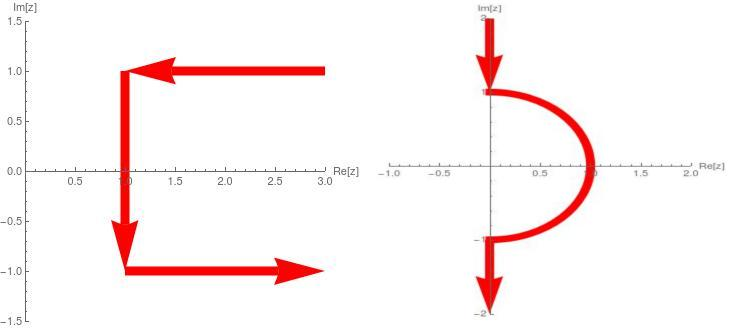
\includegraphics[scale=0.7]{contorno.jpg}
\caption{Camino tenido en cuenta para realizar la integral de contorno en el plano complejo}
\label{fig:contorno}
\end{figure}


La integral de linea puede descomponerse en 3 partes, un contorno circular y dos lineas rectas, la contribución circular es regular para todo s, entonces no aporta a la estructura de polos, en cuanto a las contribuciones del lado recto voy a realizar mi integral en funcion de t, parametrizando z de la forma $z = \pm i L t$ entonces se pueden expresar ambas integrales (luego de tirar los terminos exponencialmente decrecientes)como  (\ref{contorno}) .

\begin{equation}
    \frac{Sin(\pi s)}{ \pi } L ^{-2s+1}
    \int _1 ^{\infty} 
    t ^{-2s}
    \underbrace
    {
	\frac{ \frac{1}{L} + \gamma + \gamma t}
	{1+ t}
	} _{\chi}
    dt 
\label{contorno}
\end{equation}

Luego voy a desarrollar asintoticamente  $\chi$  (\ref{eq:chi}), para despues insertarlo en (\ref{contorno} da como resultado y realizar la integral termino a termino para luego obtener (\ref{eq.zeta.com})

\begin{equation}
    \chi = \gamma + \frac{1}{L} \sum _{n=1} ^{\infty} \frac{(-1) ^{n+1}}{t ^n}
\label{eq:chi}
\end{equation}

\begin{equation}
    \zeta _A (s) = 
    \frac{Sin(\pi s)}{\pi} L ^{1-2s}
    \left(
    \frac{\gamma}{2s+1} + 
    \sum _{n=1} ^{\infty}
    \frac{(-1) ^{n+1}}{2s-n-1}
    \right)
\label{eq.zeta.com}
\end{equation}

Donde Los primeros estan dados por 

\begin{equation}
\begin{array}{c}

\zeta(s) \approx 

\end{array}
\end{equation}

\section{Calculo del Heat-Kernel}
